\documentclass[supercite]{HustGraduPaper}

\title{基于双线性池化注意力机制的步态识别网络}
\author{古效朋}
\school{计算机科学与技术}
\classnum{ACM1501}
\stunum{U201714555}
\instructor{另一个人}
\date{2021年6月6日}

\usepackage{algorithm, multirow}
\usepackage{algpseudocode}
\usepackage{amsmath}
\usepackage{amsthm}
\usepackage{framed}
\usepackage{mathtools}
\usepackage{subcaption}
\usepackage{xltxtra} %提供了针对XeTeX的改进并且加入了XeTeX的LOGO, 自动调用xunicode宏包(提供Unicode字符宏)
\usepackage{bm}
\usepackage{tikz}
\usepackage{tikzscale}
\usepackage{pgfplots}

\pgfplotsset{compat=1.16}

\newcommand{\cfig}[3]{
  \begin{figure}[htb]
    \centering
    \includegraphics[width=#2\textwidth]{images/#1.tikz}
    \caption{#3}
    \label{fig:#1}
  \end{figure}
}

\newcommand{\sfig}[3]{
  \begin{subfigure}[b]{#2\textwidth}
    \includegraphics[width=\textwidth]{images/#1.tikz}
    \caption{#3}
    \label{fig:#1}
  \end{subfigure}
}

\newcommand{\xfig}[3]{
  \begin{figure}[htb]
    \centering
    #3
    \caption{#2}
    \label{fig:#1}
  \end{figure}
}

\newcommand{\rfig}[1]{\autoref{fig:#1}}
\newcommand{\ralg}[1]{\autoref{alg:#1}}
\newcommand{\rthm}[1]{\autoref{thm:#1}}
\newcommand{\rlem}[1]{\autoref{lem:#1}}
\newcommand{\reqn}[1]{\autoref{eqn:#1}}
\newcommand{\rtbl}[1]{\autoref{tbl:#1}}

\algnewcommand\Null{\textsc{null }}
\algnewcommand\algorithmicinput{\textbf{Input:}}
\algnewcommand\Input{\item[\algorithmicinput]}
\algnewcommand\algorithmicoutput{\textbf{Output:}}
\algnewcommand\Output{\item[\algorithmicoutput]}
\algnewcommand\algorithmicbreak{\textbf{break}}
\algnewcommand\Break{\algorithmicbreak}
\algnewcommand\algorithmiccontinue{\textbf{continue}}
\algnewcommand\Continue{\algorithmiccontinue}
\algnewcommand{\LeftCom}[1]{\State $\triangleright$ #1}

\newtheorem{thm}{定理}[section]
\newtheorem{lem}{引理}[section]

\colorlet{shadecolor}{black!15}

\theoremstyle{definition}
\newtheorem{alg}{算法}[section]

\def\thmautorefname~#1\null{定理~#1~\null}
\def\lemautorefname~#1\null{引理~#1~\null}
\def\algautorefname~#1\null{算法~#1~\null}

\begin{document}

\maketitle

\pagenumbering{roman}
\statement

\clearpage

\pagenumbering{Roman}

\begin{cnabstract}{中文关键词;中文关键词;中文关键词}

主要写面临的问题,至少占4行。不能出现``本文''、``论文''、``本课题''、``本研究''等字样。需要改变措辞,比如,``既然存在这些问题,而哪些技术针对这些问题取得了很好的效果,那么,可以采用哪些技术,从哪些方面展开研究。具体如下:''中文摘要。中文摘要。中文摘要。中文摘要。中文摘要。中文摘要。中文摘要。

解决的方法及动机不少于10行。中文摘要。中文摘要。中文摘要。中文摘要。中文摘要。中文摘要。中文摘要。中文摘要。中文摘要。中文摘要。中文摘要。中文摘要。中文摘要。中文摘要。中文摘要。中文摘要。中文摘要。中文摘要。中文摘要。中文摘要。中文摘要。中文摘要。中文摘要。中文摘要。中文摘要。中文摘要。中文摘要。中文摘要。中文摘要。中文摘要。中文摘要。中文摘要。中文摘要。中文摘要。中文摘要。中文摘要。中文摘要。中文摘要。中文摘要。中文摘要。中文摘要。中文摘要。中文摘要。中文摘要。中文摘要。中文摘要。中文摘要。中文摘要。中文摘要。中文摘要。中文摘要。中文摘要。中文摘要。中文摘要。中文摘要。中文摘要。中文摘要。中文摘要。中文摘要。中文摘要。中文摘要。中文摘要。

达到的主客观性能占4行。中文摘要。中文摘要。中文摘要。中文摘要。中文摘要。中文摘要。中文摘要。中文摘要。中文摘要。中文摘要。中文摘要。中文摘要。中文摘要。中文摘要。中文摘要。中文摘要。中文摘要。中文摘要。中文摘要。中文摘要。中文摘要。中文摘要。

\begin{enumerate}
	\renewcommand{\labelenumi}{\theenumi)}
	\item C++
	\item Java
	\item HTML
\end{enumerate}

\end{cnabstract}

\begin{enabstract}{keyword in English, keyword in English, keyword in English}

Gait recognition is a kind of long-distance biometric identification technology which can determine the identity of a person by his walking posture. It has great potential in police investigation, security and self-service. The traditional research mainly focuses on the method of manual feature extraction, which will lose part of the gait information, and the model is relatively complex.With the development of deep learning, end-to-end modeling and multi-layer feature extraction have achieved good applications in gait recognition research, but the recognition accuracy is still limited by cross-view recognition, clothing, carrying conditions and other factors.

This paper summary the development and limitations of gait recognition methods based on deep learning. As for fine-grained feature extraction, the paper learn recent searches using bilinear pooling to extract the fine-grained features, I proposed a novel bilinear pooling attention mechanism. I combined the new mechanism with gait recognition based on the existed network GaitSet proposed by Chao et al. The biliniear pooling mechanism fuse features in different channels while two attention modules enhance the most distinguished features and fuse the first-order and the second-order features. Gait recognition model with such mechanism can extract more details.

The model was tested on the public cross-view gait dataset CASIA-B. The results show that, under the same experimental conditions, the overall accuracy of gait recognition network is improved, and the accuracy under bag-carrying conditions has reached 88.6\%, leading the baseline GaitSet by a margin of 2.8\%.


\end{enabstract}

\tableofcontents[level=2]
\clearpage

\pagenumbering{arabic}

\section{绪论}
\textcolor{blue}{引用的论文\cite{wenxian}}

第一章不要少于4页。

这份模板根据\url{https://github.com/skinaze/HUSTPaperTemp}\cite{ski17}修改,添加了一些CS人常用的东西\cite{baf96}。

我是绪论。我是绪论。我是绪论。我是绪论。我是绪论。我是绪论。我是绪论。我是绪论。我是绪论。我是绪论。我是绪论。我是绪论。我是绪论。我是绪论。我是绪论。我是绪论。

\subsection{课题背景}

如何添加参考文献?先在文件夹里的bib文件里添加新的参考文献,给每篇参考文献取一个索引的名字,然后再引用比如\cite{STR2021Neurocom}\cite{AVS2021Neurocom, Rezaei2014CVPR}。请注意书籍、期刊论文、专利等bib条目的格式是不一样的。我是第一小节。我是第一小节。我是第一小节。我是第一小节。我是第一小节。我是第一小节。我是第一小节。我是第一小节。我是第一小节。我是第一小节。我是第一小节。我是第一小节。我是第一小节。我是第一小节。我是第一小节。我是第一小节。我是第一小节。我是第一小节。请注意,当正文中出现1) 2) 3)罗列时,请必须用enumerate环境,具体如下!

\begin{enumerate}
	\renewcommand{\labelenumi}{\theenumi)}
	\item C++
	\item Java
	\item HTML
\end{enumerate}

\subsubsection{研究背景和趋势}

我是第二小节。我是第二小节。我是第二小节。我是第二小节。我是第二小节。我是第二小节。我是第二小节。我是第二小节。我是第二小节。我是第二小节。我是第二小节。我是第二小节。我是第二小节。我是第二小节。我是第二小节。我是第二小节。我是第二小节。我是第二小节。中文摘要。
当正文中出现1) 2) 3)时需要用枚举环境。

\subsubsection{面临的问题和挑战}

\subsection{国内外研究现状}

\subsection{研究目的和主要内容}

参考文献无法显示怎么办?陈老师正在想办法解决\cite{STR2021Neurocom, AVS2021Neurocom}!

我是参考文献。我是第二小节\cite{Mehrabian1974An}。我是第二小节\cite{Rezaei2014CVPR}。我是第二小节\cite{Ramnath2008IJCV}。我是第二小节。我是第二小节。我是第二小节。我是第二小节。我是第二小节。我是第二小节。我是第二小节。我是第二小节。我是第二小节。我是第二小节。我是第二小节。我是第二小节。李白斗酒诗百篇 \footnote{人生得意须尽欢可能不是李白说的, 而是李白喝酒时候听酒友们说得}。

\subsection{论文结构}

\newpage

\section{必要性与可行性分析}
\textcolor{blue}{苏轼\ref{Sushi}}


念奴娇$\bullet$赤壁怀古 \\
大江东去,浪淘尽,千古风流人物。故垒西边,人道是,三国周郎赤壁。乱石穿空,惊涛拍岸,卷起千
堆雪。江山如画,一时多少豪杰。 
遥想公瑾当年,小乔初嫁了,雄姿英发。羽扇纶巾,谈笑间,樯橹灰飞烟灭。故国神游,多情应笑我,
早生华发。人生如梦,一尊还酹江月。 

\begin{figure}[ht]
	\begin{center}
		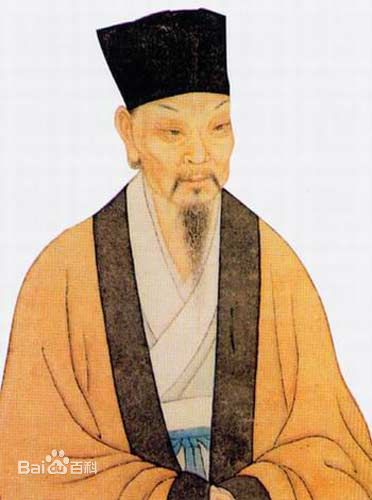
\includegraphics{Sushi.jpg}
		\caption{苏轼}
		\label{Sushi}
	\end{center}
\end{figure}


第二章不要少于5页。

\subsection{什么是必要性}

为什么要解决这个问题,有什么动机,解决了有哪些好处\cite{LTE2015MIP}?目前的方法还有什么缺陷?这是一个算法。这是一个算法。这是一个算法。这是一个算法。这是一个算法。这是一个算法。这是一个算法。这是一个算法。这是一个算法。这是一个算法。这是一个算法。这是一个算法。这是一个算法。这是一个算法。这是一个算法。

\begin{shaded*}\begin{alg}{不要用这个算法因为标准算法需要三条线条}
  \label{alg:apb}
  \begin{algorithmic}
    \Input Two numbers $a$ and $b$
    \Output The sum of $a$ and $b$
    \Procedure{A-Plus-B}{$a, b$}
      \If $a = 0$
        \State \Return $b$
      \EndIf
      \State $res \gets 0$
      \While{$b \neq 0$}
        \State Increase $res$ by $1$
        \State $b \gets b - 1$
      \EndWhile
      \State \Return $res$
    \EndProcedure
  \end{algorithmic}
\end{alg}\end{shaded*}

\begin{thm} \label{thm:gsb-apprx}
  \ralg{apb}所示的算法是正确的。
\end{thm}
\begin{proof}[证明]
  显然,此处略去。
\end{proof}

我是字。我是字。我是字。我是字。我是字。我是字。我是字。我是字。我是字。我是字。我是字。我是字。我是字。我是字。我是字。我是字。我是字。我是字。我是字。我是字。我是字。我是字。我是字。我是字。我是字。我是字。我是字。我是字。

\subsection{什么是可行性}

凭什么说能解决这些问题\cite{MIH2010IEEE}?有哪些现成理论和技术手段可以借鉴?它们为什么可以用于问题的解决?这是一张表。这是一张表。这是一张表。这是一张表。这是一张表。这是一张表。这是一张表。这是一张表。这是一张表。这是一张表。这是一张表。这是一张表。这是一张表。这是一张表。这是一张表。这是一张表。

\begin{generaltab}{表格前后不留白. 通过调整代码调整位置. 但不要让表出所在的章.}{tbl:hmm}
  \begin{tabular}{c|ccc}
    \toprule
    我是字 & 第二列 & 第三列 & 第四列 \\
    \midrule
    第一行 & $1$ & $1$ & $4$ \\
    第二行 & $5$ & $1$ & $4$ \\
    \bottomrule
  \end{tabular}
\end{generaltab}

\rtbl{hmm}是有味道的。

我是字。我是字。我是字。我是字。我是字。我是字。我是字。我是字。我是字。我是字。我是字。我是字。我是字。我是字。我是字。我是字。我是字。我是字。我是字。我是字。我是字。我是字。我是字。我是字。我是字。我是字。我是字。我是字。

如果实验报告中要用到算法伪代码,请参考\ralg{apb},也可以参考\ralg{apb}。如果实验报告中要用到伪代码,请参考\ralg{apb},也可以参考\ralg{apb}。如果实验报告中要用到算法伪代码,请参考\ralg{apb},也可以参考\ralg{apb}。如果实验报告中要用到算法伪代码,请参考\ralg{apb},更提倡参考算法\ref{alg:2}。请注意:我校的算法一般只提倡三线的形式,即算法\ref{alg:2}。如果采用了\ralg{apb},可能被指导老师答辩老师审稿老师尅!

\begin{algorithm}[h] 
	\caption{一个更复杂算法}
	\begin{algorithmic}[1]
		\State Initialization: $I_{xy}$, $z_{f}=Zeros(128, 128)$; 
		\For{$0\leq n \textless N$}
		\State $i=\lfloor x_n \rfloor+64$, $j=\lfloor y_n \rfloor + 64$
		\If{$z_n<0$ and $|z_n|>|z_{f}(i,j)|$};
		\State $z_{f}(i,j)=z_n$;
		\EndIf
		\State $I_{xy}(i,j)=z_{f}(i,j)$;
		\EndFor 
	\end{algorithmic}\label{alg:2}
\end{algorithm}

\subsection{第四章性能测试要针对第一第二章提出的问题展开}

这是一堆\cite{Dai2008Semantic}表。这是一堆表。这是一堆表。这是一堆表。这是一堆表。这是一堆表。这是一堆表。这是一堆表。这是一堆表。这是一堆表。这是一堆表。这是一堆表。这是一堆表。这是一堆图。这是一堆图。这是一堆图。

\begin{figure}[htb]
	\setlength{\abovecaptionskip}{ 0.0cm}
	\setlength{\belowcaptionskip}{-0.5cm}
	\begin{center}
		\includegraphics[scale=0.25]{Fig2-1.pdf}
		\caption{调整图的位置, 以免留白, 但图不能跑出所在的章.}
		\label{fig2-1}
	\end{center}
\end{figure}

\xfig{bpg-l}{两张小图}{
  \sfig{bpg-la}{0.3}{小图}
  \sfig{bpg-lb}{0.3}{小图}
}

图\ref{fig2-1}很好看,因为采用的是pdf格式的矢量图。\rfig{bpg-la}和\rfig{bpg-lb}因为缩得太小了不那么好看,可以在visio里把他们画在一排,就可以不用xfig命令了。我是字。我是字。我是字。我是字。我是字。我是字。我是字。我是字。我是字。我是字。我是字。我是字。我是字。我是字。我是字。我是字。我是字。我是字。我是字。我是字。我是字。我是字。我是字。我是字。我是字。我是字。我是字。我是字。

\subsection{本章小结}

\newpage

\section{总体架构与功能模块设计}
\textcolor{blue}{公式一\ref{gongshi1}}
\begin{align}
	f(x)&=4(x+3)^2-4 \nonumber\\
	&=4x^2=24x+36 
	\label{gongshi1}
\end{align}
\textcolor{blue}{公式二\ref{gongshi2}}
\begin{eqnarray}
	S=\int_{a}^{b}f(x)dx=\sum_{i=1}^{n}\frac{f(x_i)+f(x_i+1)}{2}h\approx\{\frac{1}{2}(f(a)+f(b))+\sum_{i=1}^{n-1}f(x_i)\}h 
	\label{gongshi2}
\end{eqnarray}
 
 
第三章不要少于6页\cite{STR2021Neurocom}。我是字。我是字。我是字。我是字。我是字。我是字。我是字。我是字。我是字。我是字。我是字。我是字。我是字。我是字。我是字。我是字。我是字。我是字。我是字。我是字。我是字。我是字。我是字。我是字。我是字。我是字。我是字。我是字。

\subsection{翻译主要靠有道怎么办}

我是字\cite{MU-MIMO2009IEEE}。我是字。我是字。我是字。我是字。我是字。我是字。我是字。我是字。我是字。我是字。我是字。我是字。我是字。我是字。我是字。我是字。我是字。我是字。我是字。我是字。我是字。我是字。我是字。我是字。我是字。我是字。我是字。具体方法请见公式\ref{equ_attention}

\begin{eqnarray}\label{equ_attention}
	\textbf{Y}_I=\textbf{X}_I{\odot}\textbf{A}_I,~\textbf{Y}_D=\textbf{X}_D{\odot}\textbf{A}_D %\nonumber
\end{eqnarray}

\subsection{不会找文献怎么办}

\begin{figure}[htb]
	\setlength{\abovecaptionskip}{ 0.0cm}
	\setlength{\belowcaptionskip}{-0.5cm}
	\begin{center}
		\includegraphics[scale=0.25]{Fig3-1.pdf}
		\caption{调整图的位置, 以免留白, 但图不能跑出所在的章.}
		\label{fig3-1}
	\end{center}
\end{figure}

图\ref{fig3-1}很好看,因为采用的是pdf格式的矢量图。我是字。我是字。我是字。我是字。我是字。我是字。我是字。我是字。我是字。我是字。我是字。我是字。我是字。我是字。我是字。我是字。我是字。我是字。我是字。我是字。我是字。我是字。我是字。我是字。我是字。我是字。我是字。我是字。

\subsection{看不懂英文文献怎么办}

我是字。我是字。我是字。我是字。我是字。我是字。我是字。我是字。我是字。我是字。我是字。我是字。我是字。我是字。我是字。我是字。我是字。我是字。我是字。我是字。我是字。我是字。我是字。我是字。我是字。我是字。我是字。可以按照公式\ref{equ_GMP}解决之。

\begin{eqnarray}\label{equ_GMP}
	\begin{cases}
		\textbf{G}_I=\mathrm{GMP}(\textbf{L}_I) + \mathrm{GAP}(\textbf{L}_I)\\
		\textbf{G}_D=\mathrm{GMP}(\textbf{L}_D) + \mathrm{GAP}(\textbf{L}_D)
	\end{cases}
\end{eqnarray}{}

\subsection{不会用Visio画思维导图怎么办}

我是字。$a\stackrel{<}{=}c$我是字。我是字。我是字。我是字。我是字。我是字。我是字。我是字。我是字。我是字。我是字。我是字。我是字。我是字。我是字。我是字。我是字。我是字。我是字。我是字。我是字。我是字。我是字。我是字。我是字。我是字。我是字。

\begin{table}
	\begin{center}
		\setlength{\tabcolsep}{2.0mm}
		\caption{Mean and standard deviation of estimation error (Euler angles) on Pandora. The best performance is in \textbf{bold}.}
		\label{table2}
		\begin{tabular}{c|ccccc}
			\hline
			Method    			        & Data               & Pitch         & Roll           & Yaw              & Accuracy\\
			\hline
			\hline			
			\multirow{5}{*}{POSEidon}   & Depth              & 6.5 $\pm$ 6.6  & 5.4 $\pm$ 5.1  & 10.4 $\pm$ 11.8  & 0.646\\
			                            & FfD              	 & 6.8 $\pm$ 7.0  & 5.7 $\pm$ 5.7  & 10.5 $\pm$ 14.6  & 0.647\\
			                            & Gray-level         & 7.1 $\pm$ 6.6  & 5.6 $\pm$ 5.8  & 9.0  $\pm$ 10.9  & 0.639\\
			                            & Depth + FfD	     & 5.6 $\pm$ 5.0  & 4.9 $\pm$ 5.0  & 9.8  $\pm$ 13.4  & 0.698\\
		 	                            & Depth + FfD + MI   & 5.7 $\pm$ 5.6  & 4.9 $\pm$ 5.1  & 9.0  $\pm$ 11.9  & 0.715\\
			\hline
			DRF                         & Depth              & 6.2 $\pm$ 9.5  & 4.6 $\pm$ 6.7  & 9.3  $\pm$ 14.6  & --\\
			\hline
			\multirow{3}{*}{Ours}   	& Depth              & 5.9 $\pm$ 6.2  & 4.5 $\pm$ 4.9  & 8.8  $\pm$ 10.9  & 0.666\\
			                            & RGB                & 5.5 $\pm$ 5.3  & 4.4 $\pm$ 5.5  & 8.6  $\pm$ 9.3   & 0.698\\
			                            & RGB + Depth        & 5.0 $\pm$ 4.8  & 4.3 $\pm$ 4.9  & 8.1  $\pm$ 8.3   & \textbf{0.737}\\
			\hline
		\end{tabular}
	\end{center}
\end{table}

\subsection{本章小结}

\newpage


\section{功能模块实现与性能分析}





第四章不要少于7页\cite{Multiplexing2000USA}。其中,性能分析不要少于2页。我是字。我是字。我是字。我是字。我是字。我是字。我是字。我是字。我是字。我是字。我是字。我是字。我是字。我是字。我是字。我是字。我是字。我是字。我是字。我是字。我是字。我是字。我是字。我是字。我是字。我是字。我是字。我是字。其实吧,用Latex写公式也不是很难,请参照公式\ref{equ_loss}

\begin{eqnarray}\label{equ_loss}
	\mathcal{L}_{id}=\sum_{j=1}^{c}1\{l_k=j\}\log\frac{\exp(f_j(\textbf{W},x_k))}{\sum\nolimits_{l=1}^{c}\exp(f_l(\textbf{W},x_k))}
\end{eqnarray}
\textcolor{blue}{表格\ref{table_eval}}
\begin{table}
	\begin{center}
		\setlength{\tabcolsep}{5.0mm}
		\caption{Sample Tabular: cline and hline.}
		\begin{tabular}{|l|c|r|}
			\hline 
			\multicolumn{3}{|c|}{Sample Tabular}\\
			\hline 
			col head & col head & col head\\
			\hline 
			left & center & right\\
			\cline{1-2}
			aligned & items & aligned\\
			\cline{2-3}
			items & items & items\\
			\cline{1-2}
			left & center & right\\
			\hline
			
		\end{tabular}\label{table_eval}
		
	\end{center}
\end{table}



\subsection{程序调不通怎么办}


\begin{figure}[htb]
	\setlength{\abovecaptionskip}{ 0.0cm}
	\setlength{\belowcaptionskip}{-0.5cm}
	\begin{center}
		\includegraphics[scale=0.65]{Fig4-1.pdf}
		\caption{调整图的位置, 以免留白, 但图不能跑出所在的章.}
		\label{fig4-1}
	\end{center}
\end{figure}

图\ref{fig4-1}很好看,因为采用的是pdf格式的矢量图。看网贴、问同学,也可以尝试问老师\cite{Euro2015WG}。我是字。我是字。我是字。我是字。我是字。我是字。我是字。我是字。我是字。我是字。我是字。我是字。我是字。我是字。我是字。我是字。我是字。我是字。我是字。我是字。我是字。我是字。我是字。我是字。我是字。我是字。我是字。我是字。

%\begin{align}
%	f(x) &=4(x+3)^2-4\\
%	&=4x^2+24x+36
%\end{align}

\subsection{依赖包装不了怎么办}


我是字。我是字。我是字。我是字。我是字。我是字。我是字。我是字。我是字。我是字。我是字。我是字。我是字。我是字。我是字。我是字。我是字。我是字。我是字。我是字。我是字。我是字。我是字。我是字。我是字。我是字。我是字。我是字。

%\begin{table}
%	\begin{center}
%		\setlength{\tabcolsep}{5.0mm}
%		\caption{Sample Tabular: cline and hline.}
%		\begin{tabular}{|l|c|r|}
%			\hline
%			\multicolumn{3}{|c|}{Sample Tabular}\\
%			\hline
%			col head  &  col head  & col head\\
%			\hline
%			left      &  center    & right\\
%			\cline{1-2}
%			aligned   & items      & aligned\\
%			\cline{2-3}
%			items     & items      & items\\
%			\cline{1-2}
%			left      & center     & right\\
%			\hline
%		\end{tabular}\label{table_eval}
%	\end{center}
%\end{table}

\subsection{环境变量配置不好怎么办}

%\begin{eqnarray}\label{equ_int}
%	\mathcal{S}=\int_{a}^{b}f(x)dx=\sum_{i=1}^{n}\frac{f(x_i)+f(x_{i+1})}{2}h\approx\begin{Bmatrix}\frac{1}{2}(f(a)+f(b))+\sum_{i=1}^{n-1}f(x_i)\end{Bmatrix}h
%\end{eqnarray}

我是字。我是字。我是字。我是字。我是字。我是字。我是字。我是字。我是字。我是字。我是字。我是字。我是字。我是字。我是字。我是字。我是字。我是字。我是字。我是字。我是字。我是字。我是字。我是字。我是字。我是字。我是字。我是字。

\subsection{性能比不过SoTA怎么办}


有人认为,对于本科生性能至少要比两年前的主流方法(顶会顶刊上的)要高\cite{STR2021Neurocom}!硕士研究生要比1年前的主流方法(顶会顶刊上的)的性能要高。我是字。我是字。我是字。我是字。我是字。我是字。我是字。我是字。我是字。我是字。我是字。我是字。我是字。我是字。我是字。我是字。我是字。我是字。我是字。我是字。我是字。我是字。我是字。我是字。我是字。我是字。我是字。我是字。

\subsection{贴代码}

尽量不要贴代码,最好写成算法的伪代码形式。如果一定要贴代码,那就仿照如下:

\noindent
/* Linear Table On Sequence Structure */\\
\#include <stdio.h>\\
\#include <malloc.h>\\
\#include <stdlib.h>\\

\noindent
/*---------page 10 on textbook ---------*/\\
\#define TRUE 1\\
\#define FALSE 0\\
\#define OK 1\\
\#define ERROR 0\\
\#define INFEASTABLE -1\\
\#define OVERFLOW -2\\

\subsection{本章小结}

\newpage

\section{总结与展望}

第五章不要少于2页。我是字。我是字。我是字。我是字。我是字。我是字。我是字。我是字。我是字。我是字。我是字。我是字。我是字。我是字。我是字。我是字。我是字。我是字。我是字。我是字。我是字。我是字。我是字。我是字。我是字。我是字。我是字。我是字。

\subsection{所做工作的总结}

我是字。我是字。我是字。我是字。我是字。我是字。我是字。我是字。我是字。我是字。我是字。我是字。我是字。我是字。我是字。我是字。我是字。我是字。我是字。我是字。我是字。我是字。我是字。我是字。我是字。我是字。我是字。我是字。

\subsection{存在的问题与展望}

我是字。我是字。我是字。我是字。我是字。我是字。我是字。我是字。我是字。我是字。我是字。我是字。我是字。我是字。我是字。我是字。我是字。我是字。我是字。我是字。我是字。我是字。我是字。我是字。我是字。我是字。我是字。我是字。

\subsection{字数不够怎么办}

深刻理解设计与实现中的要点并做深入展开。我是字。我是字。我是字。我是字。我是字。我是字。我是字。我是字。我是字。我是字。我是字。我是字。我是字。我是字。我是字。我是字。我是字。我是字。我是字。我是字。我是字。我是字。我是字。我是字。我是字。我是字。我是字。我是字。

\subsection{查重不过怎么办}

提高自己的写作能力!

\newpage

\begin{thankpage}

感谢陈遇落雁导师给予我的支持,提供双线性池化注意力机制的优化方案,将实验室基于双线性池化注意力机制的视野识别的研究成果给予我做参考。感谢老师提供了机器学习的服务器,提供了步态识别网络的测试环境。还要感谢老师的监督,对每一个学生,每一个任务环节都细心耐心的指导。

感谢和我一起完成实验的同学,在我刚刚接触深度学习的时候,帮助我学习机器学习的代码,为我讲解我不明白的地方。

感谢我的父母,在没有课程的时日里,监督我正常作息,日复一日坚持完成毕业设计。

感谢学院里的监督和指导,感谢学校提供了优良的学习氛围。


\end{thankpage}

\nocite{*} %% 作用是不对文献进行引用,但可以生成文献列表

\bibliographystyle{HustGraduPaper}
\bibliography{HustGraduPaper}

\setcounter{secnumdepth}{0}
\appendix

\section{附录A 本科期间承担或参与大创项目列表}

如果没有请删掉相关代码!或者用\%符号注释

\newpage
\section{附录B 本科期间发表学术论文列表}

如果没有请删掉相关代码!

\end{document}
